% !TEX encoding = UTF-8 Unicode
% !TEX root = ../Rapport/rapport.tex


Nous avons décidé d'implémenter tous les algorithmes suivants en langage C pour des raisons d'efficacité.

\section{Programmation dynamique}
La programmation dynamique est un paradigme d'algorithmes exacts qui consiste à plonger le problème dans sa généralisation. Le principe est d'utiliser une fonction de récursion pour calculer la solution optimale d'un sous-problème du problème courant. À partir de la solution de ce sous-problème, on obtient la solution d'un sous-problème plus grand, etc, jusqu'à résoudre le problème de départ. Ainsi, tous les calculs sont effectués une et une seule fois.

%Espace de recherche, sous-ensemble de l'espace de recherche

\subsection{Problème de la partition}

\subsubsection{Description du problème}
Le problème de la 2-partition de $n$ objets consiste à trouver deux sous-ensembles de ces $n$ objets tel que chacun des sous-ensembles ait le même poids. Les poids de chacun des objets étant des valeurs entières, pour qu’il existe deux sous-ensembles distincts ayant le même poids, il faut que la somme des poids des objets soit paire.

\subsubsection{Algorithme de programmation dynamique}
Prenons l'algorithme de résolution présenté dans la section théorique (cf \ref{solvepart}) et rappelé ci-dessous. Cet algorithme est un algorithme exact admettant une complexité en $O(n.P)$ avec $n$ le nombre d'objets et $P$ la somme des poids de tous les objets.
\begin{algorithm}[H]
	\caption{solve-partition}
	\begin{algorithmic}[1]
		\STATE $P \leftarrow \sum_{i \in \mathbb{[}1, n \mathbb{]}} p(a_i)$
		\IF{$P \equiv 1 \pmod{2}$}
			\STATE Pas de solutions
		\ELSE
			\FOR {$j \in \mathbb{[}0,P/2\mathbb{]}$}
				\IF{$j = 0$}
					\STATE $T(0, j) \leftarrow \TRUE$
				\ELSE
					\STATE $T(0, j) \leftarrow \FALSE$
				\ENDIF
			\ENDFOR
			\FOR{$i \in \mathbb{[}1, n \mathbb{]}$}
				\FOR{$j \in \mathbb{[}0, P/2\mathbb{]}$}
					\STATE $T(i, j) \leftarrow [\left (j = 0) \vee (j = p(a_i)) \vee (T(i-1, j)) \vee (T(i-1, j-p(a_i))) \right]$
				\ENDFOR
			\ENDFOR
			\IF{$T(n, P / 2) = \FALSE$}
				\STATE Pas de solutions
			\ELSE
				\STATE Construire le sous ensemble solution
			\ENDIF
		\ENDIF
	\end{algorithmic}
\end{algorithm}

\subsubsection{Tests}

\begin{figure}[H]
	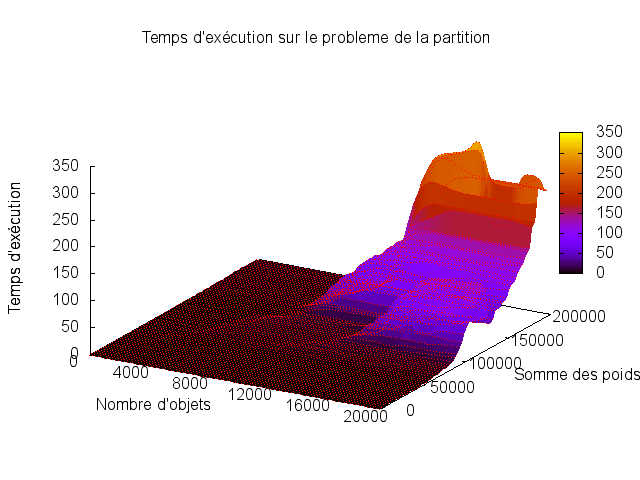
\includegraphics[width=\linewidth]{../pratique/prog_dynamique_dev/res/partition.png}
\end{figure}


\subsection{Problème du sac à dos}

\subsubsection{Description du problème}
Le problème du sac à dos consiste à vouloir mettre des objets ayant chacun différents volumes et utilités dans un sac à dos à volume limité. Le but est d'obtenir un sac à dos rempli avec une utilité maximum.

\subsubsection{Algorithme de programmation dynamique}
Prenons l'algorithme de résolution présenté ci-dessous. Cet algorithme est un algorithme exact admettant une complexité en $O(n.V^2)$ avec $n$ le nombre d'objets et $V$ le volume du sac à dos. Notons que la borne (pire des cas) est atteinte si tous les objets sont de volume 1.
\begin{algorithm}[H]
	\caption{sac à dos}
	\begin{algorithmic}[1]
		\FOR {$j \in \mathbb{\{}1, \ldots, volumeMax \mathbb{\}}$}
				\STATE $T[0, j] \leftarrow 0$
		\ENDFOR
		\FOR{$i \in \mathbb{\{}1, \ldots, n \mathbb{\}}$}
			\FOR{$j \in \mathbb{\{}1, \ldots, volumeMax \mathbb{\}}$}
				\IF{$j \neq 1$}
					\STATE $T[i, j] \leftarrow T[i, j-1]$
				\ENDIF
				\FOR{$k \in \mathbb{\{}0, \ldots, volumeMax/volume[i] \mathbb{\}}$}
					\STATE $T[i,j] \leftarrow \max(T[i,j], T[i-1,j-k \times volume[i]] + k \times utilite[i])$
				\ENDFOR
			\ENDFOR
		\ENDFOR
	
	\RETURN $T[n,volumeMax]$
	\end{algorithmic}
\end{algorithm}


\subsubsection{Tests}

\begin{figure}[H]
	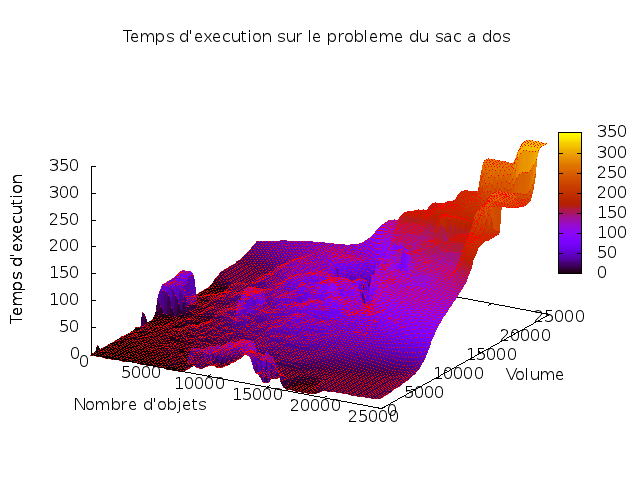
\includegraphics[width=\linewidth]{../pratique/prog_dynamique_dev/res/bag.png}
\end{figure}


\subsection{Problème du voyageur de commerce}

\subsubsection{Description du problème}
Le problème du voyageur de commerce consiste à trouver un cycle hamiltonien de poids minimum.
\subsubsection{Algorithme de programmation dynamique}

\begin{algorithm}[H]
	\caption{TSP}
	\begin{algorithmic}[1]
		\FOR {$i \in \mathbb{\{}1, \ldots, n-1 \mathbb{\}}$}
			\STATE $MeilleureChaine(\{v_i\},v_i) = (v_0, v_i)$
			\STATE $ValeurChaine(\{v_i\},v_i) = d(v_0, v_i)$
		\ENDFOR
		\FOR{$j \in \mathbb{\{}1, \ldots, n-2 \mathbb{\}}$}
			\FOR{$V^{'} \subseteq \mathbb{\{ } v_1, \ldots, v_{n-1} \mathbb{ \} } : |V^{'}|=j$}
				\FOR{$v \in V^{'}$}
					\STATE $ValeurChaine(V^{'},v) = \min\limits_{w \in V^{'}}\{ValeurChaine(V^{'}\backslash \{v\},w)+d(w,v)\}$
					\STATE $MeilleureChaine(V^{'},v) = (MeilleureChaine(V^{'}\backslash \{v\},w_0),v)$ (où $w_0$ est le sommet qui atteint ce minimum)
				\ENDFOR
			\ENDFOR
		\ENDFOR
		
		\RETURN $T=arg \min\limits_{v=v_2}^{v_n}(ValeurChaine(\{v_1,\ldots,v_{n-1}\}\backslash \{v\},v)+d(v,v_0))$
	\end{algorithmic}
\end{algorithm}


\subsubsection{Tests}

\begin{figure}[H]
	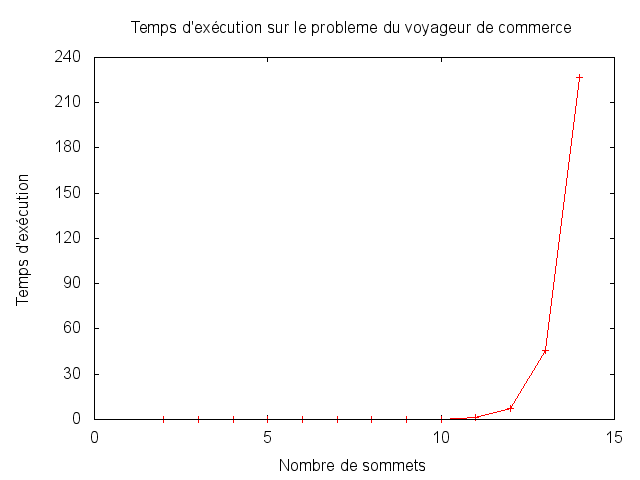
\includegraphics[width=\linewidth]{../pratique/prog_dynamique_dev/res/tsp.png}
\end{figure}


